\section{基于场景的设计和测试过程}
\label{process}
%
%The ISO~26262 standard from 2016 \cite{ISO_26262_2011} represents the state of the art for developing vehicle guidance systems with regard to functional safety\footnote{The overall system development for vehicle guidance systems includes additional parallel development processes, which cover other aspects like function development.}.
2016年出版的ISO~26262标准展示了车辆引导系统开发过程中的功能安全技术。\footnote{车辆引导系统整系统的开发包括额外平行开发流程,其涵盖功能开发等其他方面。}
%An overview of the development process proposed in the ISO~26262 standard is shown in Fig.~\ref{fig:ISO-Prozess}.
ISO~26262标准提出的开发流程如图~\ref{fig:ISO-Prozess}所示。
%The process steps which may utilize scenarios to generate the demanded work products are highlighted in red.
利用场景生成所需工作产品的过程步骤在图中以红色方框标出。
%Scenarios may support the whole development process of the ISO~26262 standard from the concept phase via the technical product development through to the system verification and validation. 
场景可以支持ISO~26262标准的整个开发过程,从概念阶段到技术产品开发,再到系统验证和测试。
%In the development process of the ISO~26262 standard scenarios may be utilized from the concept phase via the technical product development through to the system verification and validation. 
%Hence, it is mandatory to define the requirements on scenarios resulting from the different process steps. 
%These requirements allow a consistent definition of abstraction levels for the use of scenarios throughout the whole development lifecycle. 
%The following sections refer to the work products of the development process defined by the ISO~26262 standard and derive requirements on scenarios for the highlighted process steps.
因此,必须定义不同流程步骤产生的场景需求。
而在整个开发周期中,要求在不同抽象级别上对所用场景有一致性表述。
以下部分涉及ISO~26262标准定义的开发过程的工作产品,并推导出各流程的场景需求。

\begin{figure*}
	\centering
	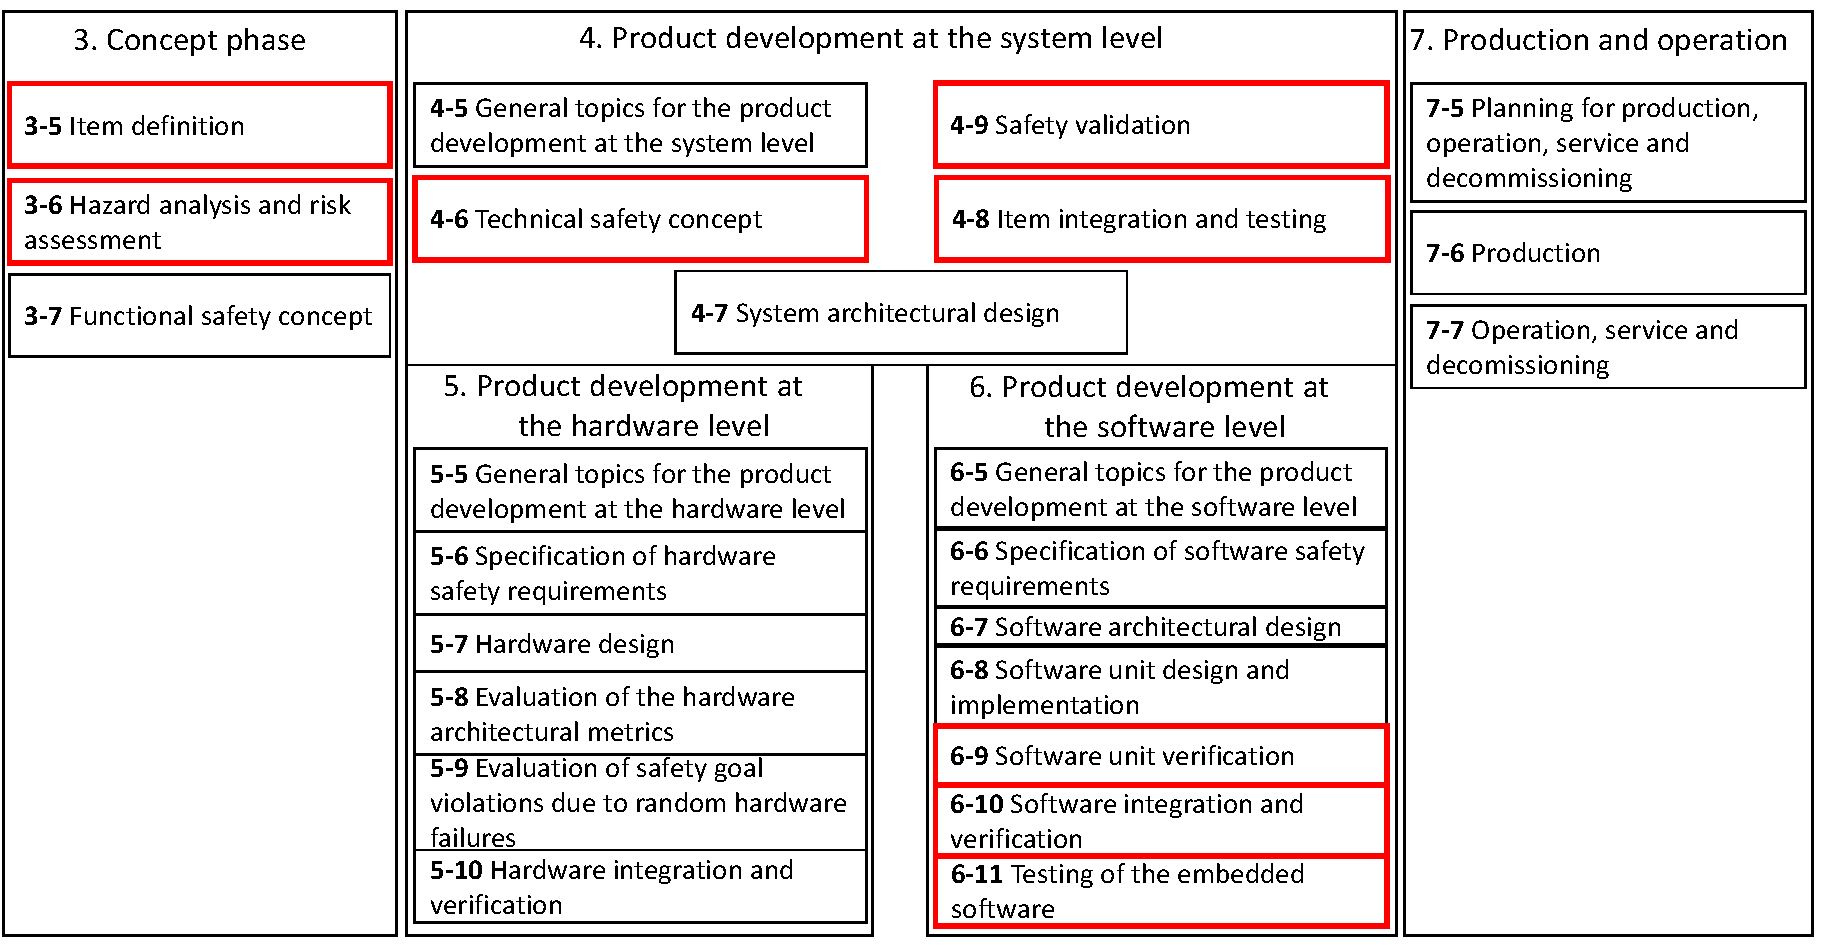
\includegraphics[width=\textwidth]{./3_process/graphics/ISO_Prozess}
	\caption{ISO~26262标准中提出的开发过程概述。红色显示的流程步骤可以利用方案来生成工作产品。}
	\label{fig:ISO-Prozess}
\end{figure*}

\subsection{概念阶段的场景}
%Prior to the technical development, the concept for the item under development is specified.
%During the concept phase of the ISO~26262 standard (part 3) the item is defined, a hazard analysis and risk assessment is conducted, and a functional safety concept is developed.
在标准第3部分的概念阶段,该标准对项目进行了定义,进行了危险分析和风险评估,并引出功能安全概念。

%The item definition shall include a description of the functional concept, system boundaries, the operational environment, the legal requirements, and the dependencies on other items.
项目定义包括功能定义、系统边界、操作环境、法规需求以及对其他项目的依赖关系的描述。基于这些信息,可以派生出可能的操作场景。
%Based on this information, possible operating scenarios can be derived. 
%Reschka \cite{Reschka2016} proposes to identify safe driving states and specify the nominal behavior based on the operating scenarios.
Reschka\cite {Reschka2016}建议识别安全驾驶状态,并根据操作场景指定名义行为。
%The operating scenarios in this process step shall be described in an abstract level of detail and be represented in a human understandable way (textual description).
此过程中的操作场景应以较抽象的方式描述,并以一种易于理解的方式表示。
%The next process step defined by the ISO~26262 standard which uses scenarios is the hazard analysis and risk assessment.
由ISO~26262标准定义的下一个使用场景的过程步骤是危害分析和风险评估。
%The hazard analysis and risk assessment consists of two steps: the situation analysis and the hazard identification, and the classification of hazardous events.
危害分析和风险评估包括两个步骤:情景分析和危险识别,以及危险事件的分类。
%In the situation analysis, all operational situations\footnote{The authors point out that the term `operational situation' as it is used in the ISO~26262 standard should be declared as `operational scenario' according to Ulbrich~et~al.~\cite{ulbrich_definition_2015}.} and operating modes in which malfunctioning behavior will result in a hazardous event shall be described.
在情况分析中,所有操作情况\footnote{作者指出,根据Ulbrich等人的说法,ISO~26262标准中使用的术语“操作情况”应该被称为“操作情景”。 \cite{ulbrich_definition_2015}。}和导致危险事件的故障行为中的操作模式均需要描述。
%Whereby, malfunctioning behavior can be interpreted as deviation from the specified nominal behavior.
%Afterwards, hazardous scenarios, which include a combination of operational scenarios and malfunctioning behavior, will be rated using the automotive safety integrity level (ASIL). 
因此,故障行为可以理解为偏离指定的正常行为。之后,将使用汽车安全完整性等级(ASIL)对危险情景进行评级,其中包括操作情景和故障行为的组合。
%\todo{AR: Geagte These: Ich muss ohnehin alle Szenarien untersuchen, wenn ich es strukturiert und vollständig machen möchte und mich nicht nur auf %Expertenwissen beziehen möchte.}
%The parameters for the ASIL classification are the exposure of the operational scenario, the possible severity, and the controllability of the hazardous scenario\footnote{The controllability of a scenario includes the controllability by the driver/passenger of the automated vehicle and the controllability by other traffic participants.}.
ASIL分类的参数是操作场景的暴露程度,可能的严重程度以及危险场景的可控性\footnote{场景的可控性包括自动驾驶车辆的驾驶员/乘客的可控性以及其他车辆的可控性 交通参与者}。
%In order to determine these parameters, the description of hazardous scenarios has to include the stationary surroundings (scenery) and all traffic participants which may interact with the automated vehicle.
为了确定这些参数,危险场景的描述必须包括静止环境(场景)和可以与自动驾驶车辆交互的所有交通参与者。
%According to the actual state of the art, the analysis of hazardous scenarios is performed by experts. 
%Hence, hazardous scenarios have to be formulated in natural language.
根据现有技术,危险情景的分析由专家进行。因此,必须以自然语言制定危险情景。
%Depending on their area of expertise, human experts vary in the level of detail regarding the terms they use to describe a scenario.
根据他们的专业领域,人类专家在用于描述场景的术语方面的细节水平各不相同。
%Thus, a unified vocabulary for the functional perspective during the process step of the hazard analysis and risk assessment is necessary.
因此,在危害分析和风险评估的过程步骤中,功能视角的统一词汇表是必要的。
%Furthermore, to ensure a common understanding among the experts, the terms within the vocabulary have to be organized in a semi-formal way.
此外,为了确保专家之间的共同理解,词汇表中的术语必须以半正式的方式组织。
%In this way, it is possible to combine vocables from the vocabulary and generate scenarios.
%These scenarios are expressed by language and have a minimal room for interpretation.

%Scenarios have to fulfill the following requirements to be utilized during the concept phase [C] of the ISO~26262 standard:
在ISO~26262标准的概念阶段[C],场景必须满足以下需求:
\begin{itemize}
	\item[C1] 人类专家应该能够用自然语言来描述该场景。
	\item[C2] 场景应以半正式的方式表示。
\end{itemize}


\subsection{系统开发阶段的场景}
%Once the hazardous scenarios have been analyzed, a functional safety concept is developed.
%To implement the functional concept, technical safety requirements have to be derived in process step 4-6.
%As opposed to functional requirements, technical requirements outline criteria which can be physically quantified.
一旦分析了危险场景,就会形成功能安全概念。为了实现功能安全,须提出技术安全需求。与功能需求不同,技术安全需求描述了可量化的条件。
%can be quantified in a physical manner.
%For example, the functional requirement to keep a safe driving distance to other traffic participants can be technically formulated by a distance in meters, which has to be satisfied.
%Hence, every hazardous scenario has to be converted from the linguistic and semi-formal representation of the \textit{concept phase} to a representation via state values for the technical \textit{product development on system level} (4).
例如,保持与其他交通参与者的安全驾驶距离的安全需求通过以米为单位的距离来确定。因此,每个危险场景都必须从半正式的自然语言表述(概念阶段)转换为利用状态量表述(系统开发阶段)的方式。
%A list of those state variables is a precise description of a scenario, but, due to the high level of detail, not intuitively processable by human experts.
这些状态量的列表是对场景的精确描述,但由于细节水平抽象程度高,人类专家无法直观地处理这些状态量。
%To reduce the quantity of scenarios, state values can be summarized in value ranges. 
%Later on, those value ranges can be further detailed in valid/invalid ranges to define a set of safe and unsafe values respectively, or to model the system boundaries.
为了减少场景的数量,可以给定状态量的取值范围,或者可以进一步划分有效/无效的取值范围,即安全/不安全的取值,从而明确系统边界。场景的详细表述确保了能以可验证的方式制定开发项目的需求。
%A detailed representation of scenarios ensures that the requirements on the item to be developed can be formulated in a verifiable way.
方案的详细表述确保了可以以可验证的方式制定对待开发项目的需求。
%This is a necessary condition for the safety validation in process step 4-9 of the ISO~26262 standard.
这是ISO~26262标准的步骤4-9中的安全验证的必要条件。
%All in all, scenarios have to fulfill the following requirements to be utilized during the system development phase [S] of the ISO~26262 standard:
总而言之,场景必须满足ISO~26262标准的系统开发阶段[S]中要使用的以下需求:
\begin{itemize}
	\item[S1] 场景应包括用于场景表示的状态量的参数范围。
	\item[S2] 场景应为每项参数指定一个标记,以支持自动处理。
\end{itemize}

\subsection{测试与验证阶段的场景}
%During the test phase, it is examined whether the implemented system fulfills the requirements specified in the previous process steps.
在测试阶段,将验证系统是否满足了前述流程中指定的需求。
%For this verification, the tests have to be systematically planned, specified, executed, evaluated, and documented \cite[part 8, section 9.2]{ISO_26262_2011}.
这一过程,验证必须依据标准\cite[part 8, section 9.2]{ISO_26262_2011},系统地计划、制定、执行、评估和记录。
%Each test case specification has to include the following information independently from the test method \cite[part 8, section 9.4.2]{ISO_26262_2011}:
每个测试用例规范必须独立于测试方法包括以下信息\cite[part 8, section 9.4.2]{ISO_26262_2011}:
\begin{enumerate}
\item  一个独特的标识
\item 要验证的工作产品的引用参考
\item 前提条件和配置\footnote{在系统变体的意义上。}
\item 环境条件
\item 输入数据,包括它们的时间顺序
\item 预期的行为,包括可接受的变化
\end{enumerate}

%A very challenging aspect of the test case generation is the specification of input data.
测试用例生成的一个难点在于输入数据的规范性,包括每个参数的时间序列,这些时间序列实质上影响测试对象的行为。
%This data has to include time sequences of each parameter which is essentially affecting the behavior of the test object.
%At the same time, due to highly connected systems, the input data may not contain any inconsistencies\footnote{Unintended inconsistencies are meant here. Fault injections can be utilized as a test method later on.}, but rather represent a consistent scenario.
同时,由于高度连接的系统,输入数据可能不包含任何不一致\footnote{这里不一致的意思:故障注入可以在以后用作测试方法。},而是代表一致的场景。
%Information regarding the operational environment of the system under verification as well as possible operating scenarios are already given in the item definition, which is specified during the concept phase of the development process according to the ISO~26262 standard.  
概念阶段已经给出了系统的操作环境和可能的操作场景,这是为测试用例派生一致的输入数据的基础
%Based on this information, consistent input data can be derived for the specification of test cases.
%The scenarios used in the item definition are expressed by language and formulated on an abstract level of detail. 
项目定义中使用的场景由语言表达,并在抽象的详细程度上制定。
%To utilize these abstract scenarios within the scope of a test case, the scenarios have to be specified in detail and concretized.
要在测试用例的范围内使用这些抽象场景,必须详细指定场景并使其具体化。
%The detailed specification of scenarios can be performed within the scope of the \textit{specification of technical safety requirements} \cite[part 4, section 6]{ISO_26262_2011}.
场景的详细规范可以在技术安全需求规范的范围内进行\cite[part 4, section 6]{ISO_26262_2011}.
%The technical safety requirements describe how the item has to react to external stimuli which can affect the compliance with the safety goals.
技术安全要求描述了项目如何对可能影响安全目标的外部影响做出反应。
%The technical requirements specify the linguistic requirements 
%In this way, the technical requirements also define for which parameter ranges the functionality of the system under development has to be ensured.
通过这种方式,技术要求还定义了必须确保正在开发系统的功能参数范围。
%This parameter space has to be tested during the verification process and thus has to be taken into account for the test case generation.
必须在验证过程中测试该参数空间,因此必须考虑该生成测试用例。
%In addition, the scenarios have to be converted to a formal representation during the step of specifying the scenarios in detail.
%A formal representation is necessary, to ensure a reproducible test case execution later on.
此外,还必须将场景转换为正式表达,以确保之后测试用例的可执行性及可复现性。
%To ensure a reproducible test case execution later on, a formal representation is necessary.
%The scenarios have to define all parameters required for test case execution via different test methods (like simulation or field tests).
场景必须通过不同的测试方法(如模拟或现场测试)定义测试用例执行所需的所有参数。
%Thus, in the step of specifying a scenario in detail, a conversion has to be conducted from an informal description based on organized terms to a formal description based on physical system state values.
因此,在详细指定场景的步骤中,必须从基于有组织的术语的非正式描述到基于物理系统状态值的形式描述进行转换。
%To generate the input data included in a test case, discrete parameter values have to be chosen from the continuous parameter ranges of a specified scenario in a concretization step.
为了生成测试用例的输入数据,必须从指定场景的连续参数范围中选择离散参数值。
%Schuldt \cite{Schuldt2017} proposes the use of equivalence classes, boundary value analysis, and combinatorial methods for identifying representative samples.
Schuldt \cite{Schuldt2017}提出使用等价类,边界值分析和组合方法来识别代表性样本。
%This approach provides a systematic generation of test cases, but lacks a method to determine a meaningful test coverage.
这种方法提供了系统生成的测试用例,但缺乏确定有意义的测试覆盖率的方法。
%For determining a meaningful test coverage, the test concept, the scenario selection, and the necessary test methods have to be taken into account.
为了确定有意义的测试覆盖率,必须考虑测试概念,场景选择和必要的测试方法。
%The scenarios, which are systematically derived during the concretization step and then formally described, represent consistent input data for the item under test.
在具体步骤中系统地导出,然后正式描述的场景代表被测系统的一致输入数据。
%Thus, the derived scenarios can be used in the scope of a test case for the verification of the implemented system.
因此,派生的场景可以在测试用例的范围内用于验证所实现的系统。
%All in all, scenarios have to fulfill the following requirements to be utilized during the testing phase [T] of the ISO~26262 standard:
总而言之,场景必须满足ISO~26262标准的测试阶段[T]中要使用的以下要求:

\begin{itemize}
	\item[T1] 场景应该通过具体的状态值来描述,以确保其可执行性和可复现性。
	\item[T2] 场景应具备一致性。
	\item[T3] 场景应该以一种高效的机器可读的方式表示,以确保自动化测试的执行。
\end{itemize}

\subsection{对场景需求的分析}
%Table \ref{tab:contradictoryRequirements} illustrates that the specified requirements are contradictory regarding the form of scenario description. 
表\ref {tab:contradictoryRequirements}说明了指定的要求与场景描述的矛盾。
%On the one hand, requirement C1 states the demand for an abstract, linguistic scenario representation and, on the other hand, requirements S2 and T3 state the demand for an efficient, machine readable scenario representation.
一方面,需求概念阶段C1表示对抽象的语言场景表示的需求,另一方面,需求S2和T3表示对有效的机器可读场景表示的需求。
%Since linguistic representations are hard to process by machines and human beings are not able to read size efficient (mostly binary coded) data formats, there is a demand for different forms of scenario representations.
由于语言表示很难由机器处理,并且人类无法读取大小有效(主要是二进制编码)的数据格式,因此需要不同形式的场景表示。
%Similarly, requirements S1 and T2 demand different levels of detail for the scenario representation.
类似地,S1和T2场景需求表示的不同细节程度。
%On the one hand, requirement S1 asks for a scenario representation via parameter ranges in the state space. 
一方面,需求S1通过状态空间中的参数范围来表述场景。
%This form of representation offers multiple degrees of freedom regarding the determination of concrete values to be tested.
这种表示形式在确定要测试的具体值方面提供了多个自由度。
%On the other hand, requirement T2 asks for a representation that includes concrete parameter values. 
另一方面,需求T2要求包括具体参数值来表述需求。
%This form of representation is required for a reproducible test case execution.
这是测试用例可重复执行的必要条件
%Hence, machine readable scenarios have to support two different levels of detail.
因此,机器可读的场景必须支持两种不同的细节程度。

\begin{table*}
	\centering
	\caption{场景需求的矛盾 ($\perp$ 矛盾标记)}
	\label{tab:contradictoryRequirements}
	\begin{tabularx}{\textwidth}{ X l X l X }
		\hline \\
		概念阶段 & & 系统开发阶段 & & 测试阶段 \\
		\hline \\
	人类专家应能够用自然语言制定该领域的术语。 & \multirow{3}{4pt}{$\perp$} &  场景应包括用于场景表述的状态值的参数范围。 & \multirow{3}{4pt}{$\perp$} & 场景应通过具体的状态值建模,以确保其可重复性并能够使测试方法执行场景。 \\
		\hline \\
	\end{tabularx}
\end{table*}
